\documentclass[usenames,dvipsnames,10pt,aspectratio=169]{beamer} 
% Add option 'aspectratio=169' for 16:9 widescreen 
% Add option  'handout' to ignore animations
% If you have a smaller amount of text, feel free to also try '11pt'! / Jesper

\usepackage[utf8]{inputenc}
\usepackage{verbatim}
\usepackage{minted}
\usemintedstyle{monokai}
\usepackage{graphicx}
\usepackage{wrapfig}
\usepackage[document]{ragged2e}
\usetheme{umu}

%%% Bibliography
\usepackage[style=authoryear,backend=biber]{biblatex}
\addbibresource{bibliography.bib}

\DeclareNameAlias{author}{given-family}

%%% Suppress biblatex annoying warning
\usepackage{silence}
\WarningFilter{biblatex}{Patching footnotes failed}

%%% Some useful commands
% pdf-friendly newline in links
\newcommand{\pdfnewline}{\texorpdfstring{\newline}{ }} 
% Fill the vertical space in a slide (to put text at the bottom)
\newcommand{\framefill}{\vskip0pt plus 1filll}

%%% Enter additional packages below (or above, I can't stop you)! / Jesper
\renewcommand{\proofname}{\sffamily{Proof}}

%%%%%%%%%%%%%%%%%%%%%%%%%%%%%%%%%%%%%%%%%%%%%%%%%%%%%%%%%%%%%%%%%%%%%%%%%%%%%%%%%%%%%
\title[Rust \#1]{Rust \#1: Motivation and Introduction}
\date[\today]{\small\today}
\author[Sultanov Andriy]{Sultanov Andriy}
\institute{APPS@UCU}

\begin{document}

\begin{frame}
\titlepage
\end{frame}

\begin{frame}{\contentsname}
\tableofcontents
\end{frame}

\framepic{graphics/1.jpg}{
 \textcolor{ucuwhite}{A short history of systems programming}
 \vskip 0.5cm
 }

\section{A short history of systems programming}
\begin{frame}{The origins of C}

\begin{wrapfigure}{r}{0.5\textwidth}
\centering
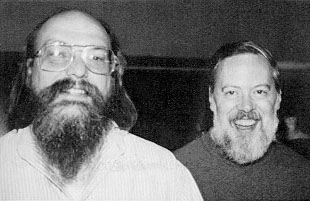
\includegraphics[width=0.5\textwidth]{graphics/ritchie.jpg}
\end{wrapfigure}
The C programming language appeared during Unix development in 1972.\\

Since it was created for a specific purpose % an operating system
and a specific computer %(PDP-11) 
, on one hand it adapted to the
needs of the programmers, and on the 
other hand it adopted a large
amount of somewhat unique and unpopular 
ideas and concepts.
%  Since it’s basically assembly, you are 
%  operating on the naked memory, with almost 
%  no abstractions (everything is either 
%  just a naked data or a pointer to naked 
%  data). This produces several problems:
%  Hard to write more or less 
%  complex programs because the language 
%  itself provides a small number of 
%  abstractions and libraries

\vskip 0.8cm

\end{frame}

\begin{frame}{Possible solutions}

C++ is born to help address some of these problems, 
introduces ‘zero cost’ abstractions, aimed 
at providing a nice interface for the 
programmer to use which compiles down to 
an almost ideal machine code. 

Still has the old instruments %(the fucking BACKWARDS COMPATIBILITY), 
and tries to enforce using the new modern
safe instruments%(which are ugly in their own ways)
, which is not ideal. Continues to hang on 
to C’s model of the machine and programming itself.


\end{frame}

\begin{frame}{Modern ideas}

On the other hand, languages like Java, 
Ruby and Python start sprawling up, 
presenting another model of growth - 
they are garbage-collected and are able 
to present even more complex abstractions 
without programmers having so much headache, 
and without any high speed expectations.

Go and others try to address C’s problem, unsuccessfully.

\end{frame}

\framepic{graphics/1.jpg}{
 \textcolor{ucuwhite}{Pitfalls of the old ways}
 \vskip 0.5cm
 }

\section{Pitfalls of the old ways}

\begin{frame}{General stuff} 
	General stuff about how they are not memory-safe.
	

	Should probably spend some time explaining the memory layout,
	so it'd be possible to explain buffer overflows, dangling 
	pointers and null pointers.sasasjasa
\end{frame}

\begin{frame}{Buffer overflows} 
	\inputminted[fontsize=\large]{c}{code/overflow.c}
\end{frame}

\begin{frame}{Null pointers}
	\inputminted[fontsize=\large]{c}{code/nullp.c}
\end{frame}

\begin{frame}{Dangling pointers} 
	\inputminted[fontsize=\large]{c}{code/danp.c}
\end{frame}

\begin{frame}{Invalidated iterators} 
	\inputminted[fontsize=\large]{c}{code/iter.c}
\end{frame}

\begin{frame}{No real error checking} 
	\inputminted[fontsize=\large]{c}{code/errorcheck.c}
\end{frame}

\begin{frame}{And many more...}
	\begin{enumerate}
		\item Memory leak - you can forget to free data
		\item Thread unsafety - another function can be modifying the same memory
		\item Double free - you can free the same memory twice (as a part of a struct, for example)
	\end{enumerate}
\end{frame}


\framepic{graphics/1.jpg}{
 \textcolor{ucuwhite}{Where and why is Rust better?}
 \vskip 0.5cm
 }

\section{Where and why is Rust better?}

\begin{frame}{What is Rust?} 
A modern system programming language.

Uses the slogan "Safe, Fast, Easy to write. Choose three"

Gets rid of unnecessary old ideas, combining them
with some of the fresh concepts.
\end{frame}

\begin{frame}{Almost everything makes sense} 
It does not care about C’s old ways 
from the 70s which have been kept up 
in many languages and systems since 
just because (null-char strings, pointers) 
and does not try to needlessly attach new 
stupid things to it. Easily gets rid of bad 
ideas since it’s a young language.
\end{frame}

\begin{frame}{Memory safety guarantees} 
\end{frame}

\begin{frame}{Improvements in almost every field} 
\end{frame}

\begin{frame}{An amazing ecosystem} 
\end{frame}

\framepic{graphics/1.jpg}{
 \textcolor{ucuwhite}{Basic syntax and concepts}
 \vskip 0.5cm
 }

\section{Basic syntax and concepts}

\begin{frame}{Enumerates and itemizes}

\end{frame}

\framepic{graphics/1.jpg}{
	\textcolor{ucuwhite}{The Rust ecosystem\\ and a little more...}
 \vskip 0.5cm
 }

\section{The Rust ecosystem and a little more}

\begin{frame}{cargo}
\end{frame}

\end{document}
